\section{Программно-техническое приложение}

В данном разделе будут описаны особенности работы с суперкомпьютером НИУ ВШЭ, которые могут быть важными дополнением к основной инструкции пользователя.

\subsection{Применение jit-компиляции при программировании на языке Python}
\label{subsection:njit_problem}

Симуляции случайного блуждания с самопересечениями (для кода см. папку $Random\_Walk$  \cite{web:ProjectMagnetRepos}) были запрограммированны на языке Python с компиляцией с помощью пакета numba метод jit. В качестве окружения была использована стандартная библиотека $Python/Anaconda\_v11.2021$ встроенная в стандартное ПО суперкомпьютера. 

Выполнение первых экспериментов по симуляциям шло крайне медленно - результаты за семь дней можно увидеть на таблице \ref{tab:Ran_Walk_neigh_1}

\begin{table}[h]
    \centering
    \begin{tabular}{|c|c|c|c|c|c|c|}
        \hline
        N & $steps$ & $unique$ & $n_{1}$ & $n_{2}$ & $n_{3}$ & $n_{4}$ \\ \hline
        100 & 7450000 & 0.49(8) & 0.07(3) & 0.33(9) & 0.36(7) & 0.24(9) \\ \hline
        200 & 5684000 & 0.44(7) & 0.05(2) & 0.29(7) & 0.35(5) & 0.30(9) \\ \hline
        500 & 2045000 & 0.39(6) & 0.04(1) & 0.24(5) & 0.34(4) & 0.38(8) \\ \hline
        1000 & 654000 & 0.36(5) & 0.03(1) & 0.22(4) & 0.33(4) & 0.42(7) \\ \hline
        2500 & 132000 & 0.33(4) & 0.027(7) & 0.19(3) & 0.31(3) & 0.48(6)  \\ \hline
        5000 & 37000 & 0.31(4) & 0.024(5) & 0.17(3) & 0.29(3) & 0.51(6) \\ \hline
        10000 & 10000 & 0.29(3) & 0.021(4) & 0.16(2) & 0.28(3) & 0.54(5) \\ \hline
    \end{tabular}
    \caption{Средние доли узлов c 1-4-мя соседями в конформациях модели Random-Walk длин $10^{2}-10^{4}$}
    \label{tab:Ran_Walk_neigh_1}
\end{table}

Для сравнения с другими платформами, в случае длины цепочки $N=10000$, процесс из 10000 шагов на Google Colab занимал не более 7 часов.

\begin{figure}[h]
    \centering
    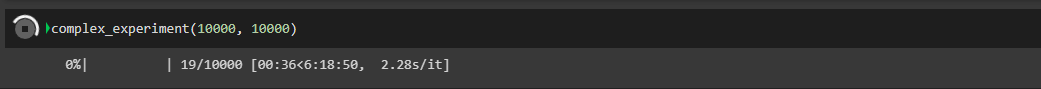
\includegraphics[width=0.95\textwidth]{experiment_time.png}
\end{figure}

Решением проблемы оказалось создание собственного окружения с другими версиями используемых пакетов numpy и numba (полный список так же есть в репозитории с кодом \cite{web:ProjectMagnetRepos}). Новые результаты за 7 дней описаны в продолжении основного раздела.

При обсуждении столь значительного различия во времени выполнениями между окружениями поддержкой было выдвинуто предположение, что окружения отличаются сторонними библиотеками линейной алгебры, используемой пакетом numpy: наиболее распространенными считаются OpenBLAS и Intel MKL. Основным фактором преимущества той или иной библиотеки является именно процессор (Intel или non-Intel). 

В новом окружении пакетом numpy использовалась именно библиотека OpenBLAS, в то время как в Anaconda - Intel MKL. Это следовало из применения в данных окружениях следующего:

\begin{code}
import numpy

print(numpy.show\_config())
\end{code}

Подробнее об определении какая библиотека линейной алгебры используется в пакете numpy можно найти \href{https://shaalltime.medium.com/benchmark-numpy-with-openblas-and-mkl-library-on-amd-ryzen-3950x-cpu-96184f91057f}{здесь}. 


\subsection{Итерации программного комплекса Rand-Walk}

Подраздел посвящён описанию версий программного комплекса для симуляций модели простого случайного блуждания фиксированной длины N на квадратной решётке.
(для кода см. папку $Random\_Walk$  \cite{web:ProjectMagnetRepos})

\begin{enumerate}
\item \textbf{Drunken\_Sailor\_def.py} - базовый алгоритм симуляций, предназначенный для проверки работы основных функций: 
\begin{itemize}
\item experiment - генерация цепочки и подсчёт наблюдаемых (доли узлов с числом соседей 1-4, а так же доля уникальных узлов цепочки)
\item \textit{complex\_experiment} - запись результирующего массива для одной цепочки (experiment) и набора цепочек (шаг - кол-во опытов между анализом данных)
\item \textit{write\_results} - запись текущих результатов (средних наблюдаемых по всем экспериментам) в текстовый файл
\item \textit{save\_distr} - распределение значений наблюдаемых по всем экспериментам
\item \textit{save\_history} - сохранение истории средний значений для анализа сходимости результаотв симуляций
\end{itemize}
Цепочка генерируется как двумерный массив точек, потому наиболее его медленной частью является поиск уникальных узлов цепочки через \textit{np.unique}, не поддерживающий njit-комплиляцию при обработке двумерного массива.
\item \textbf{Drunken\_Sailor.py} - первая версия симуляционного комплекса с jit-компилируемой частью. Алгоритмически не отличается от \textbf{Drunken\_Sailor\_def.py}, но значительно быстрее базовой версии
\item \textbf{Drunken\_Sailor\_v2.py} - оптимизированная версия \textbf{Drunken\_Sailor.py} c расширенной njit-комплиляцией:
\begin{itemize} 
\item \textit{create\_walk} - генерация цепочки как массива поворотов блуждания начиная с начальной точки $(0,0)$, затем - как массив всех точек блуждания
\item \textit{calc\_fractions} - основная функция подсчёта наблюдаемых. Так же модифицирована над подсчёт атмосферы каждого блуждания
\item В \textit{complex\_experiment} добавлено распараллеливание проведение набора экспериментов за шаг между выводом данных, что позволило значительно ускорить работу комплекса.
\item \textit{stats} - подсчёт текущего результата для наблюдаемых долей
\item \textit{atm\_bins} - подсчёт долей блужданий с атмосферой 0-3
\end{itemize}
\end{enumerate}
